\documentclass[journal,12pt,twocolumn]{IEEEtran}
\usepackage{setspace}
\usepackage{gensymb}
\usepackage{xcolor}
\usepackage{caption}
%\usepackage{subcaption}
%\doublespacing
\singlespacing
%\usepackage{graphicx}
%\usepackage{amssymb}
%\usepackage{relsize}
\usepackage[cmex10]{amsmath}
\usepackage{mathtools}
%\usepackage{amsthm}
%\interdisplaylinepenalty=2500
%\savesymbol{iint}
%\usepackage{txfonts}
%\restoresymbol{TXF}{iint}
%\usepackage{wasysym}
\usepackage{hyperref}
\usepackage{amsthm}
\usepackage{mathrsfs}
\usepackage{txfonts}
\usepackage{stfloats}
\usepackage{cite}
\usepackage{cases}
\usepackage{subfig}
%\usepackage{xtab}
\usepackage{longtable}
\usepackage{multirow}
%\usepackage{algorithm}
%\usepackage{algpseudocode}
%\usepackage{enumerate}
\usepackage{enumitem}
\usepackage{mathtools}
%\usepackage{iithtlc}
%\usepackage[framemethod=tikz]{mdframed}
\usepackage{listings}
\usepackage{polynom}

%\usepackage{wasysym}
%\newcounter{MYtempeqncnt}
\DeclareMathOperator*{\Res}{Res}
%\renewcommand{\baselinestretch}{2}
\renewcommand\thesection{\arabic{section}}
\renewcommand\thesubsection{\thesection.\arabic{subsection}}
\renewcommand\thesubsubsection{\thesubsection.\arabic{subsubsection}}

\renewcommand\thesectiondis{\arabic{section}}
\renewcommand\thesubsectiondis{\thesectiondis.\arabic{subsection}}
\renewcommand\thesubsubsectiondis{\thesubsectiondis.\arabic{subsubsection}}

%\renewcommand{\labelenumi}{\textbf{\theenumi}}
%\renewcommand{\theenumi}{P.\arabic{enumi}}

% correct bad hyphenation here
\hyphenation{op-tical net-works semi-conduc-tor}

\makeatletter
\def\pld@CF@loop#1+{%
    \ifx\relax#1\else
        \begingroup
          \pld@AccuSetX11%
          \def\pld@frac{{}{}}\let\pld@symbols\@empty\let\pld@vars\@empty
          \pld@false
          #1%
          \let\pld@temp\@empty
          \pld@AccuIfOne{}{\pld@AccuGet\pld@temp
                            \edef\pld@temp{\noexpand\pld@R\pld@temp}}%
           \pld@if \pld@Extend\pld@temp{\expandafter\pld@F\pld@frac}\fi
           \expandafter\pld@CF@loop@\pld@symbols\relax\@empty
           \expandafter\pld@CF@loop@\pld@vars\relax\@empty
           \ifx\@empty\pld@temp
               \def\pld@temp{\pld@R11}%
           \fi
          \global\let\@gtempa\pld@temp
        \endgroup
        \ifx\@empty\@gtempa\else
            \pld@ExtendPoly\pld@tempoly\@gtempa
        \fi
        \expandafter\pld@CF@loop
    \fi}
\def\pld@CMAddToTempoly{%
    \pld@AccuGet\pld@temp\edef\pld@temp{\noexpand\pld@R\pld@temp}%
    \pld@CondenseMonomials\pld@false\pld@symbols
    \ifx\pld@symbols\@empty \else
        \pld@ExtendPoly\pld@temp\pld@symbols
    \fi
    \ifx\pld@temp\@empty \else
        \pld@if
            \expandafter\pld@IfSum\expandafter{\pld@temp}%
                {\expandafter\def\expandafter\pld@temp\expandafter
                    {\expandafter\pld@F\expandafter{\pld@temp}{}}}%
                {}%
        \fi
        \pld@ExtendPoly\pld@tempoly\pld@temp
        \pld@Extend\pld@tempoly{\pld@monom}%
    \fi}
\makeatother

\lstset{
language=Python,
frame=single, 
breaklines=true,
columns=fullflexible
}

\begin{document}

\theoremstyle{definition}
\newtheorem{theorem}{Theorem}[section]
\newtheorem{problem}{Problem}
\newtheorem{proposition}{Proposition}[section]
\newtheorem{lemma}{Lemma}[section]
\newtheorem{corollary}[theorem]{Corollary}
\newtheorem{example}{Example}[section]
\newtheorem{definition}{Definition}[section]
%\newtheorem{algorithm}{Algorithm}[section]
%\newtheorem{cor}{Corollary}
\newcommand{\BEQA}{\begin{eqnarray}}
\newcommand{\EEQA}{\end{eqnarray}}
\newcommand{\define}{\stackrel{\triangle}{=}}

\bibliographystyle{IEEEtran}
%\bibliographystyle{ieeetr}

\providecommand{\nCr}[2]{\,^{#1}C_{#2}} % nCr
\providecommand{\nPr}[2]{\,^{#1}P_{#2}} % nPr
\providecommand{\mbf}{\mathbf}
\providecommand{\pr}[1]{\ensuremath{\Pr\left(#1\right)}}
\providecommand{\qfunc}[1]{\ensuremath{Q\left(#1\right)}}
\providecommand{\sbrak}[1]{\ensuremath{{}\left[#1\right]}}
\providecommand{\lsbrak}[1]{\ensuremath{{}\left[#1\right.}}
\providecommand{\rsbrak}[1]{\ensuremath{{}\left.#1\right]}}
\providecommand{\brak}[1]{\ensuremath{\left(#1\right)}}
\providecommand{\lbrak}[1]{\ensuremath{\left(#1\right.}}
\providecommand{\rbrak}[1]{\ensuremath{\left.#1\right)}}
\providecommand{\cbrak}[1]{\ensuremath{\left\{#1\right\}}}
\providecommand{\lcbrak}[1]{\ensuremath{\left\{#1\right.}}
\providecommand{\rcbrak}[1]{\ensuremath{\left.#1\right\}}}
\theoremstyle{remark}
\newtheorem{rem}{Remark}
\newcommand{\sgn}{\mathop{\mathrm{sgn}}}
\providecommand{\abs}[1]{\left\vert#1\right\vert}
\providecommand{\res}[1]{\Res\displaylimits_{#1}} 
\providecommand{\norm}[1]{\lVert#1\rVert}
\providecommand{\mtx}[1]{\mathbf{#1}}
\providecommand{\mean}[1]{E\left[ #1 \right]}
\providecommand{\fourier}{\overset{\mathcal{F}}{ \rightleftharpoons}}
\providecommand{\ztrans}{\overset{\mathcal{Z}}{ \rightleftharpoons}}
%\providecommand{\hilbert}{\overset{\mathcal{H}}{ \rightleftharpoons}}
\providecommand{\system}{\overset{\mathcal{H}}{ \longleftrightarrow}}
	%\newcommand{\solution}[2]{\textbf{Solution:}{#1}}
\newcommand{\solution}{\noindent \textbf{Solution: }}
\providecommand{\dec}[2]{\ensuremath{\overset{#1}{\underset{#2}{\gtrless}}}}
\numberwithin{equation}{section}
%\numberwithin{equation}{subsection}
%\numberwithin{problem}{subsection}
%\numberwithin{definition}{subsection}


%\renewcommand{\thefigure}{\theproblem.\arabic{figure}}
%\renewcommand{\thefigure}{\theproblem}
\renewcommand{\thefigure}{\arabic{section}.\arabic{figure}}
\makeatletter
\@addtoreset{figure}{section}
\makeatother
%\numberwithin{figure}{subsection}

\def\putbox#1#2#3{\makebox[0in][l]{\makebox[#1][l]{}\raisebox{\baselineskip}[0in][0in]{\raisebox{#2}[0in][0in]{#3}}}}
     \def\rightbox#1{\makebox[0in][r]{#1}}
     \def\centbox#1{\makebox[0in]{#1}}
     \def\topbox#1{\raisebox{-\baselineskip}[0in][0in]{#1}}
     \def\midbox#1{\raisebox{-0.5\baselineskip}[0in][0in]{#1}}

\vspace{3cm}

\title{Digital Signal Processing}

\author{Gautam Singh} 

% make the title area
\maketitle

%\newpage

\tableofcontents

%\renewcommand{\thefigure}{\thesection.\theenumi}
%\renewcommand{\thetable}{\thesection.\theenumi}

%\renewcommand{\thefigure}{\theenumi}
%\renewcommand{\thetable}{\theenumi}

%\renewcommand{\theequation}{\thesection}


\bigskip

\begin{abstract}
This manual provides a simple introduction to digital signal processing.
\end{abstract}
\noindent \section{Software Installation}
\noindent Run the following commands (commands may change depending on Linux distro)
\begin{lstlisting}
$ sudo apt update && sudo apt upgrade
$ sudo apt install libffi-dev libsndfile1 python3-scipy python3-pip python3-numpy python3-matplotlib 
$ pip3 install cffi pysoundfile 
\end{lstlisting}
\section{Digital Filter}
\begin{enumerate}[label=\thesection.\arabic*
,ref=\thesection.\theenumi]
\item
\label{prob:input}
Download the sound file using
\begin{lstlisting}
$ wget https://raw.githubusercontent.com/goats-9/ee3900-assignments/main/Assignment_01/codes/Sound_Noise.wav
\end{lstlisting}
\item
\label{prob:spectrogram}
You will find a spectrogram at \href{https://academo.org/demos/spectrum-analyzer}{\url{https://academo.org/demos/spectrum-analyzer}}. Upload the sound file that you downloaded in Problem \ref{prob:input} in the spectrogram and play. Observe the spectrogram. What do you find?

\solution There are a lot of yellow lines between 440 Hz to 5.1 KHz.  These represent the synthesizer key tones. Also, the key strokes
are audible along with background noise.
\item
\label{prob:output}
Write the python code for removal of out of band noise and execute the code.

\solution
Download the source code using
\begin{lstlisting}
$ wget https://raw.githubusercontent.com/goats-9/ee3900-assignments/main/Assignment_01/codes/2_3.py
\end{lstlisting}
and execute it using
\begin{lstlisting}
$ python3 2_3.py
\end{lstlisting}
\item
The output of the python script in Problem \ref{prob:output} is the audio file \texttt{Sound\_With\_ReducedNoise.wav}. Play the file in the spectrogram in Problem \ref{prob:spectrogram}. What do you observe?

\solution The key strokes as well as background noise is subdued in the audio. Also, the signal is blank for frequencies above 5.1 kHz.

\end{enumerate}
\section{Difference Equation}
\begin{enumerate}[label=\thesection.\arabic*,ref=\thesection.\theenumi]
\item Let
\begin{equation}
x(n) = \cbrak{\underset{\uparrow}{1},2,3,4,2,1}
\end{equation}
Sketch $x(n)$.
\item Let
\begin{multline}
\label{eq:iir_filter}
y(n) + \frac{1}{2}y(n-1) = x(n) + x(n-2), 
\\
y(n) = 0, n < 0
\end{multline}
Sketch $y(n)$.

\solution The following C code calculates $y(n)$.
\begin{lstlisting}
$ wget https://raw.githubusercontent.com/goats-9/ee3900-assignments/main/codes/3_2.c
\end{lstlisting}
Run it using
\begin{lstlisting}
$ gcc -lm -Wall -g -O2 3_2.c
$ ./a.out
\end{lstlisting}
The following code plots Fig. \eqref{fig:xnyn}.
\begin{lstlisting}
$ wget https://raw.githubusercontent.com/goats-9/ee3900-assignments/main/codes/3_2.py
\end{lstlisting}
Execute it using
\begin{lstlisting}
$ python3 3_2.py
\end{lstlisting}

\begin{figure}[!ht]
	\centering
	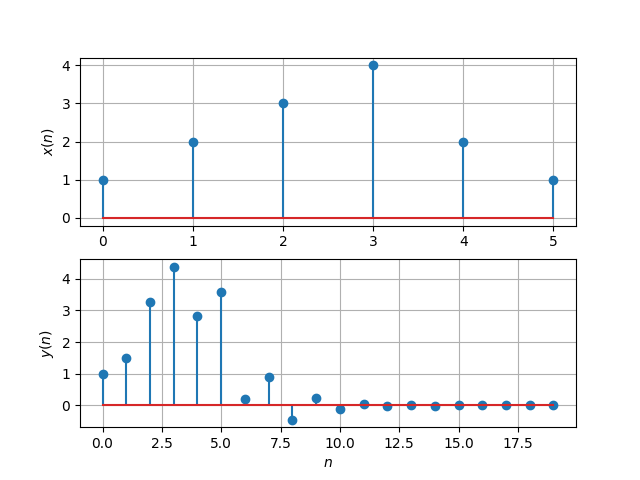
\includegraphics[width=\columnwidth]{figs/3_2.png}
	\caption{Plot of $x(n)$ and $y(n)$}
	\label{fig:xnyn}
\end{figure}
\end{enumerate}

\section{$Z$-transform}
\begin{enumerate}[label=\thesection.\arabic*]
\item The $Z$-transform of $x(n)$ is defined as
\begin{equation}
\label{eq:z_trans}
X(z)={\mathcal {Z}}\{x(n)\}=\sum _{n=-\infty }^{\infty }x(n)z^{-n}
\end{equation}
Show that
\begin{equation}
\label{eq:shift1}
{\mathcal {Z}}\{x(n-1)\} = z^{-1}X(z)
\end{equation}
and find
\begin{equation}
	{\mathcal {Z}}\{x(n-k)\} 
\end{equation}
\solution From \eqref{eq:z_trans},
\begin{align}
{\mathcal {Z}}\{x(n-k)\} &=\sum _{n=-\infty }^{\infty }x(n-k)z^{-n}\\
&=\sum _{n=-\infty }^{\infty }x(n)z^{-n-k} \\
&= z^{-k}\sum _{n=-\infty }^{\infty }x(n)z^{-n} \\
&= z^{-k}X\brak{z}
\label{eq:z_trans_shift}
\end{align}
Putting $k = 1$ gives \eqref{eq:shift1}. For the given $x(n)$, we have
\begin{align}
	X(z) &= 1 + 2z^{-1} + 3z^{-2} + 4z^{-3} \nonumber \\
		&+ 2z^{-4} + z^{-5} \\
	\implies {\mathcal {Z}}\{x(n-1)\} &= z^{-1} + 2z^{-2} + 3z^{-3} \nonumber \\
									  &+4z^{-4} + 2z^{-5} + z^{-6} \\
	&= z^{-1}X(z)
\end{align}	
\item Find
\begin{equation}
H(z) = \frac{Y(z)}{X(z)}
\end{equation}
from  \eqref{eq:iir_filter} assuming that the $Z$-transform is a linear operation.

\solution  Applying \eqref{eq:z_trans_shift} in \eqref{eq:iir_filter},
\begin{align}
Y(z) + \frac{1}{2}z^{-1}Y(z) &= X(z)+z^{-2}X(z) \\
\implies \frac{Y(z)}{X(z)} &= \frac{1 + z^{-2}}{1 + \frac{1}{2}z^{-1}}
\label{eq:freq_resp}
\end{align}

\item Find the Z transform of 
\begin{equation}
\delta(n) =
\begin{cases}
1 & n = 0 \\
0 & \text{otherwise}
\end{cases}
\label{eq:dirac-delta}
\end{equation}
and show that the $Z$-transform of
\begin{equation}
\label{eq:unit_step}
u(n) =
\begin{cases}
1 & n \ge 0 \\
0 & \text{otherwise}
\end{cases}
\end{equation}
is
\begin{equation}
U(z) = \frac{1}{1-z^{-1}}, \quad \abs{z} > 1
\end{equation}
\solution We see using \eqref{eq:dirac-delta} that
\begin{align}
	\mathcal{Z}\cbrak{\delta\brak{n}} = \delta\brak{0} = 1
\end{align}
and from \eqref{eq:unit_step},
\begin{align}
U(z) &= \sum _{n= 0}^{\infty}z^{-n} \\
&=\frac{1}{1-z^{-1}}, \quad \abs{z} > 1
\end{align}
using the fomula for the sum of an infinite geometric progression.

\item Show that 
\begin{equation}
\label{eq:anun}
a^nu(n) \ztrans \frac{1}{1-az^{-1}} \quad \abs{z} > \abs{a}
\end{equation}

\solution
\begin{align}
	a^nu(n) &\ztrans \sum_{n = 0}^{\infty}\brak{az^{-1}}^n \\
			&= \frac{1}{1-az^{-1}} \quad \abs{z} > \abs{a}
\end{align}

\item 
Let
\begin{equation}
H\brak{e^{\j \omega}} = H\brak{z = e^{\j \omega}}.
\end{equation}
Plot $\abs{H\brak{e^{\j\omega}}}$.  Comment.  $H(e^{\j \omega})$ is
known as the {\em Discrete Time Fourier Transform} (DTFT) of $h(n)$.

\solution The following code plots Fig. \eqref{fig:H-w}.
\begin{lstlisting}
$ wget https://raw.githubusercontent.com/goats-9/ee3900-assignments/main/Assignment_01/codes/4_5.py
\end{lstlisting}
The figure can be generated using
\begin{lstlisting}
$ python3 4_5.py
\end{lstlisting}
Using \eqref{eq:freq_resp}, we observe that $\left|H\brak{e^{\j\omega}}\right|$ is given by
\begin{align}
	\left|H\brak{e^{\j\omega}}\right| &= \left|\frac{1 + e^{-2\j\omega}}{1 + \frac{1}{2}e^{-\j\omega}}\right| \\
									  &= \sqrt{\frac{\brak{1 + \cos{2\omega}}^2 + \brak{\sin{2\omega}}^2}{\brak{1 + \frac{1}{2}\cos{\omega}}^2 + \brak{\frac{1}{2}\sin{\omega}}^2}}\\
									  &= \sqrt{\frac{2\brak{1 + \cos{2\omega}}}{\frac{5}{4} + \cos{\omega}}} \\
									  &= \sqrt{\frac{2\brak{2\cos^2{\omega}}}{\frac{5}{4} + \cos{\omega}}} \\
									  &= \frac{4|\cos{\omega}|}{\sqrt{5 + 4\cos{\omega}}}
\end{align}
Thus,
\begin{align}
	\left|H\brak{e^{\j\brak{\omega + 2\pi}}}\right| &= \frac{4|\cos\brak{\omega + 2\pi}|}{\sqrt{5 + 4\cos\brak{\omega + 2\pi}}} \\
											   &= \frac{4|\cos{\omega}|}{\sqrt{5 + 4\cos{\omega}}} \\
											   &= \left|H\brak{e^{\j\omega}}\right|	
\end{align}
and so its fundamental period is $2\pi$.
\begin{figure}[!ht]
	\centering
	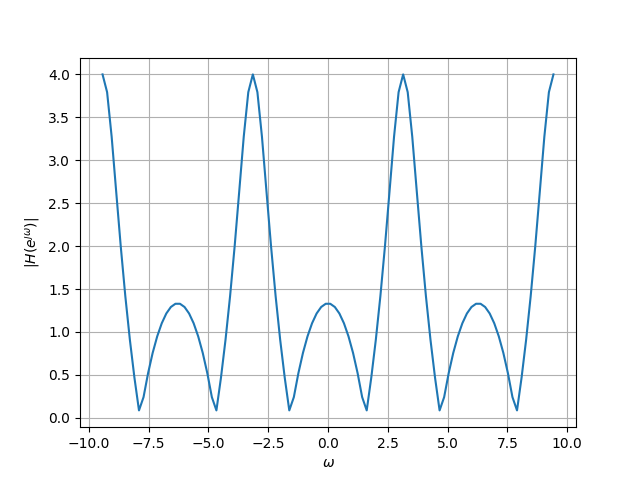
\includegraphics[width=\columnwidth]{figs/4_5.png}
	\caption{Plot of $\left|H\brak{e^{\j\omega}}\right|$ against $\omega$}
	\label{fig:H-w}
\end{figure}

\item Express $h(n)$ in terms of $H(e^{\j\omega})$.

\solution We have,
\begin{align}
	H(e^{\j\omega}) &= \sum_{k = -\infty}^{\infty}h(k)e^{-\j\omega k}
\end{align}
However,
\begin{align}
	\int_{-\pi}^{\pi}e^{\j\omega(n - k)}d\omega =
	\begin{cases}
		2\pi & n = k \\
		0 & \textrm{otherwise}
	\end{cases}
\end{align}
and so,
\begin{align}
	&\frac{1}{2\pi}\int_{-\pi}^{\pi}H(e^{\j\omega})e^{j\omega n}d\omega \\
	&= \frac{1}{2\pi}\sum_{k = -\infty}^{\infty}\int_{-\pi}^{\pi}h(k)e^{\j\omega(n - k)}d\omega \\
	&= \frac{1}{2\pi}2\pi h(n) = h(n)
\end{align}

which is known as the Inverse Discrete Fourier Transform. Thus,
\begin{align}
	h(n) &= \frac{1}{2\pi}\int_{-\pi}^{\pi}H(e^{\j\omega})e^{\j\omega n}d\omega \\
		 &= \frac{1}{2\pi}\int_{-\pi}^{\pi}\frac{1 + e^{-2\j\omega}}{1 + \frac{1}{2}e^{-\j\omega}}e^{\j\omega n}d\omega
	\label{eq:idtft}
\end{align}
\end{enumerate}

\section{Impulse Response}
\begin{enumerate}[label=\thesection.\arabic*]

\item Using long division, compute $h(n)$ for $n < 5$ from $H(z)$.

\solution We substitute $x := z^{-1}$, and perform the long division.

\polylongdiv{1 + x^2}{1 + \frac{1}{2}x}

Thus,
\begin{align}
	H(z) &= -4 + 2z^{-1} + \frac{5}{1 + \frac{1}{2}z^{-1}} \\
		 &= -4 + 2z^{-1} + 5\sum_{n = 0}^{\infty}\brak{-\frac{1}{2}}^nz^{-n} \\
		 &= 1 - \frac{1}{2}z^{-1} + 5\sum_{n = 2}^{\infty}\brak{-\frac{1}{2}}^nz^{-n} \\
		 &= \sum_{n = 0}^{\infty}\brak{-\frac{1}{2}}^nz^{-n} + 4\sum_{n = 2}^{\infty}\brak{-\frac{1}{2}}^nz^{-n} \\
		 &= \sum_{n = -\infty}^{\infty}u(n)\brak{-\frac{1}{2}}^nz^{-n} + \nonumber \\
		 &\sum_{n = -\infty}^{\infty}u(n - 2)\brak{-\frac{1}{2}}^{n - 2}z^{-n}
\end{align}

Therefore, from \eqref{eq:z_trans}, 
\begin{align}
	h(n) = \brak{-\frac{1}{2}}^{n}u(n) + \brak{-\frac{1}{2}}^{n-2}u(n-2)
\end{align}

\item \label{prob:impulse_resp}
Find an expression for $h(n)$ using $H(z)$, given that 
\begin{equation}
\label{eq:impulse_resp}
h(n) \ztrans H(z)
\end{equation}
and there is a one to one relationship between $h(n)$ and $H(z)$. $h(n)$ is known as the {\em impulse response} of the
system defined by \eqref{eq:iir_filter}.

\solution From \eqref{eq:freq_resp},
\begin{align}
H(z) &= \frac{1}{1 + \frac{1}{2}z^{-1}} + \frac{ z^{-2}}{1 + \frac{1}{2}z^{-1}} \\
\implies h(n) &= \brak{-\frac{1}{2}}^{n}u(n) + \brak{-\frac{1}{2}}^{n-2}u(n-2)
\end{align}
using \eqref{eq:anun} and \eqref{eq:z_trans_shift}.

\item Sketch $h(n)$. Is it bounded? Convergent? 

\solution The following code plots Fig. \eqref{fig:h-n}.
\begin{lstlisting}
$ wget https://raw.githubusercontent.com/goats-9/ee3900-assignments/main/Assignment_01/codes/5_2.py
\end{lstlisting}
and execute it using
\begin{lstlisting}
$ python3 5_2.py
\end{lstlisting}

\begin{figure}[!ht]
	\centering
	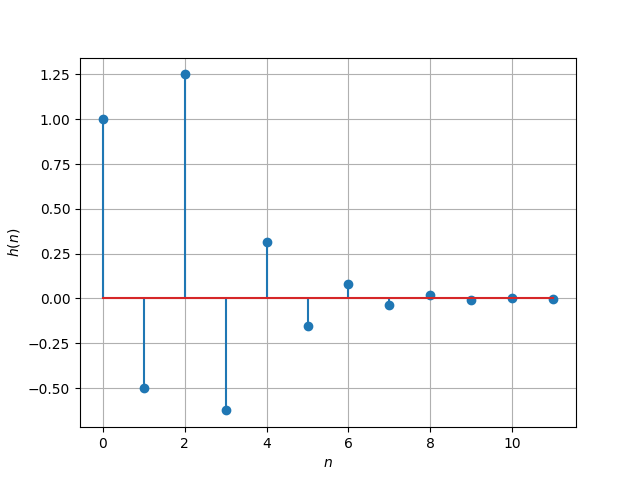
\includegraphics[width=\columnwidth]{figs/5_2.png}
	\caption{$h(n)$ as the inverse of $H(z)$}
	\label{fig:h-n}
\end{figure}
We see that $h(n)$ is bounded. For large $n$,
\begin{align}
	h(n) &= \brak{-\frac{1}{2}}^n + \brak{-\frac{1}{2}}^{n - 2} \\
		 &= \brak{-\frac{1}{2}}^{n}\brak{4 + 1} = 5\brak{-\frac{1}{2}}^n \\
		 &\implies \left|\frac{h(n + 1)}{h(n)}\right| = \frac{1}{2}
\end{align}
and therefore, $\lim_{n \to \infty}\left|\frac{h(n + 1)}{h(n)}\right| = \frac{1}{2} < 1$. Hence, we see that $h(n)$ converges.  
\item The system with $h(n)$ is defined to be stable if
\begin{equation}
\sum_{n=-\infty}^{\infty}h(n) < \infty
\end{equation}
Is the system defined by \eqref{eq:iir_filter} stable for the impulse response in \eqref{eq:impulse_resp}?

\solution
Note that
\begin{align}
	\sum_{n = -\infty}^{\infty}h\brak{n} &= \sum_{n = -\infty}^{\infty}
	\brak{-\frac{1}{2}}^nu\brak{n} + \brak{-\frac{1}{2}}^{n - 2}u\brak{n - 2} \\
										 &= 2\brak{\frac{1}{1 + \frac{1}{2}}} = \frac{4}{3}
\end{align}
Thus, the given system is stable. The limit is verified at
\begin{lstlisting}
$ wget https://raw.githubusercontent.com/goats-9/ee3900-assignments/main/Assignment_01/codes/5_3.py
\end{lstlisting}
and the code can be run using
\begin{lstlisting}
$ python3 5_3.py
\end{lstlisting}

\item 
Compute and sketch $h(n)$ using 
\begin{equation}
\label{eq:iir_filter_h}
h(n) + \frac{1}{2}h(n-1) = \delta(n) + \delta(n-2), 
\end{equation}
This is the definition of $h(n)$.

\solution The following code plots Fig. \eqref{fig:h-n-inv}. Note that this is
the same as Fig. \eqref{fig:h-n}.
\begin{lstlisting}
$ wget https://raw.githubusercontent.com/goats-9/ee3900-assignments/main/Assignment_01/codes/5_4.py
\end{lstlisting}
and executed using
\begin{lstlisting}
$ python3 5_4.py
\end{lstlisting}

\begin{figure}[!ht]
	\centering
	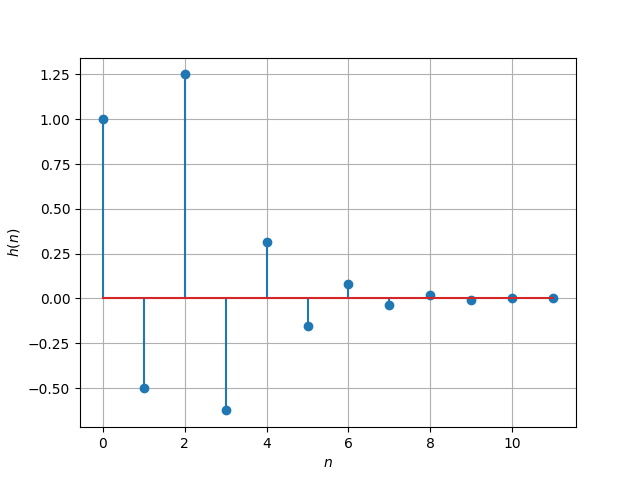
\includegraphics[width=\columnwidth]{figs/5_4.png}
	\caption{$h(n)$ as the inverse of $H(z)$}
	\label{fig:h-n-inv}
\end{figure}
\item Compute 
\begin{equation}
\label{eq:convolution}
y(n) = x(n)*h(n) = \sum_{k=-\infty}^{\infty}x(k)h(n-k)
\end{equation}

Comment. The operation in \eqref{eq:convolution} is known as
{\em convolution}.

\solution The following code plots Fig. \eqref{fig:y-n-conv}. Note that this is
the same as $y(n)$ in  Fig. \eqref{fig:xnyn}.
\begin{lstlisting}
$ wget https://raw.githubusercontent.com/goats-9/ee3900-assignments/main/Assignment_01/codes/5_5.py
\end{lstlisting}
and executed using
\begin{lstlisting}
$ python3 5_5.py
\end{lstlisting}
We use Toeplitz matrices for convolution
\begin{align}
	\mtx{y} &= \mtx{x} \circledast \mtx{h}\\
	\mtx{y} &= 
	\begin{pmatrix}
		h_1 & 0 & . & . & . & 0 \\
		h_2 & h_1 & . & . & . & 0 \\
		h_3 & h_2 & h_1 & . & . & 0 \\
		. & . & . & . & . & . \\
		0 & . & . & h_3 & h_2 & h_1 \\
		0 & . & . & . & h_2 & h_1 \\
		0 & . & . & . & 0 & h_1
	\end{pmatrix}
	\begin{pmatrix}
		x_1 \\ x_2 \\ \vdots \\ x_n
	\end{pmatrix}
\end{align}
\begin{figure}[!ht]
	\centering
	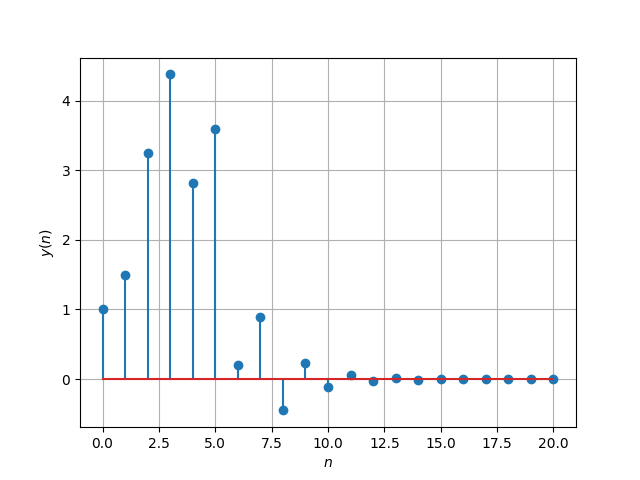
\includegraphics[width=\columnwidth]{figs/5_5.png}
	\caption{$y(n)$ from the definition}
	\label{fig:y-n-conv}
\end{figure}
\item Show that
\begin{equation}
y(n) =  \sum_{k=-\infty}^{\infty}x(n-k)h(k)
\end{equation}
\solution 
From \eqref{eq:convolution}, we substitute $k := n - k$ to get
\begin{align}
y\brak{n} &= \sum_{k=-\infty}^{\infty}x\brak{k}h\brak{n - k} \\
		  &= \sum_{n - k=-\infty}^{\infty}x\brak{n - k}h\brak{k} \\
		  &= \sum_{k=-\infty}^{\infty}x\brak{n - k}h\brak{k}
\end{align}
\end{enumerate}

\section{DFT and FFT}
\begin{enumerate}[label=\thesection.\arabic*]
\item
Compute
\begin{equation}
X(k) \define \sum _{n=0}^{N-1}x(n) e^{-\j2\pi kn/N}, \quad k = 0,1,\dots, N-1
\end{equation}
and $H(k)$ using $h(n)$.
\item Compute 
\begin{equation}
Y(k) = X(k)H(k)
\label{eq:fp}
\end{equation}
\item Compute
\begin{equation}
y\brak{n}={\frac {1}{N}}\sum _{k=0}^{N-1}Y\brak{k}\cdot e^{\j 2\pi kn/N},\quad n = 0,1,\dots, N-1
\label{eq:inv-ft}
\end{equation}

\solution The following code plots Fig. \eqref{fig:y-n-dft} and computes $X(k)$
and $Y(k)$. Note that this is the same as $y(n)$ in Fig. \eqref{fig:xnyn}.

\begin{lstlisting}
$ wget https://raw.githubusercontent.com/goats-9/ee3900-assignments/main/Assignment_01/codes/6_3.py
\end{lstlisting}
and executed using
\begin{lstlisting}
$ python3 6_3.py
\end{lstlisting}

\begin{figure}[!ht]
	\centering
	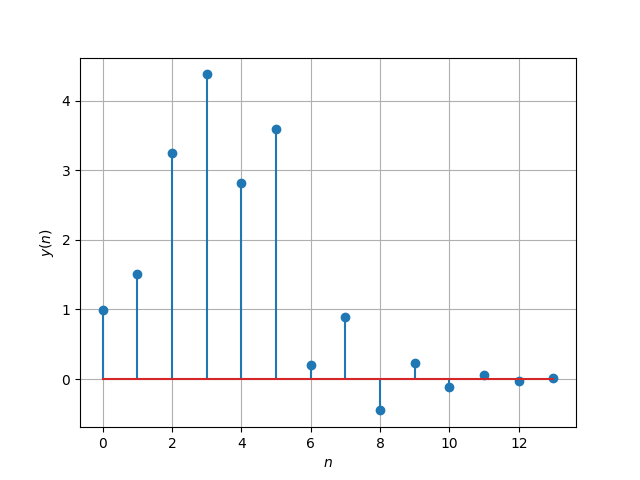
\includegraphics[width=\columnwidth]{figs/6_3.png}
	\caption{$y(n)$ from the DFT}
	\label{fig:y-n-dft}
\end{figure}
\item Repeat the previous exercise by computing $X(k), H(k)$ and $y(n)$ through FFT and 
IFFT.

\solution Download the code from
\begin{lstlisting}
$ wget https://raw.githubusercontent.com/goats-9/ee3900-assignments/main/Assignment_01/codes/6_4.py
\end{lstlisting}
and execute it using
\begin{lstlisting}
$ python3 6_4.py
\end{lstlisting}
Observe that Fig. \eqref{fig:y-n-fft} is the same as $y(n)$ in Fig. \eqref{fig:xnyn}.

\begin{figure}
	\centering
	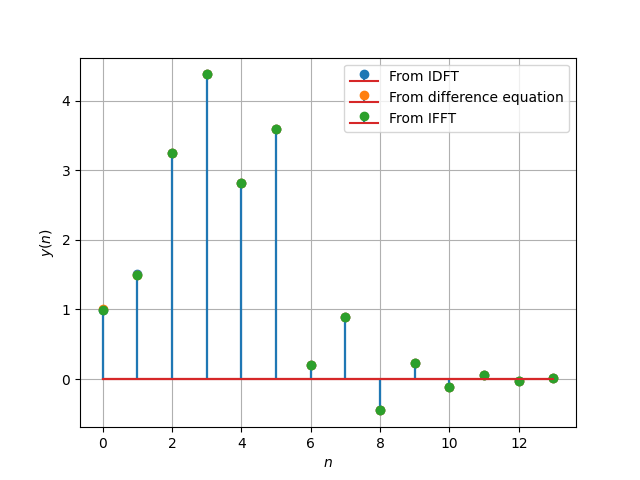
\includegraphics[width=\columnwidth]{figs/6_4.png}
	\caption{$y(n)$ using FFT and IFFT}
	\label{fig:y-n-fft}
\end{figure}
\item Wherever possible, express all the above equations as matrix equations.

\solution
We use the DFT Matrix, where $\omega = e^{-\frac{j2k\pi}{N}}$, which is given by
\begin{align}
	\mtx{W} = 
	\begin{pmatrix}
		\omega^0 & \omega^0 & \ldots & \omega^0 \\
		\omega^0 & \omega^1 & \ldots & \omega^{N - 1} \\
		\vdots & \vdots & \ddots & \vdots \\
		\omega^0 & \omega^{N - 1} & \ldots & \omega^{(N -1)(N - 1)}
	\end{pmatrix}
\end{align}
i.e. $W_{jk} = \omega^{jk}$, $0 \leq j, k < N$. Hence, we can write any DFT equation as
\begin{align}
	\mtx{X} = \mtx{W}\mtx{x} = \mtx{x}\mtx{W}
\end{align}
\noindent where
\begin{align}
	\mtx{x} = 
	\begin{pmatrix}
		x(0) \\ x(1) \\ \vdots \\ x(n - 1)
	\end{pmatrix}
\end{align}
\noindent Using \eqref{eq:inv-ft}, the inverse Fourier Transform is given by
\begin{align}
	\mtx{x} = \mathcal{F}^{-1}\brak{\mtx{X}} = \mtx{W}^{-1}\mtx{X} &= 
	\frac{1}{N}\mtx{W^{H}}\mtx{X} = \frac{1}{N}\mtx{X}\mtx{W^{H}} \\ 
	\implies \mtx{W}^{-1} &= \frac{1}{N}\mtx{W^{H}}
\end{align}
\noindent where $H$ denotes hermitian operator. We can rewrite \eqref{eq:fp} using the
element-wise multiplication operator as
\begin{align}
	\mtx{Y} = \mtx{H}\cdot\mtx{X} = \brak{\mtx{W}\mtx{h}}\cdot\brak{\mtx{W}\mtx{x}}
\end{align}
The plot of $y(n)$ using the DFT matrix in Fig. \eqref{fig:yn-mtx} is the same as $y(n)$ in 
Fig. \eqref{fig:xnyn}. Download the code using
\begin{lstlisting}
$ wget https://raw.githubusercontent.com/goats-9/ee3900-assignments/main/Assignment_01/codes/6_5.py
\end{lstlisting}
and run it using
\begin{lstlisting}
$ python3 6_5.py 
\end{lstlisting}
\end{enumerate}

\begin{figure}[!htb]
	\centering
	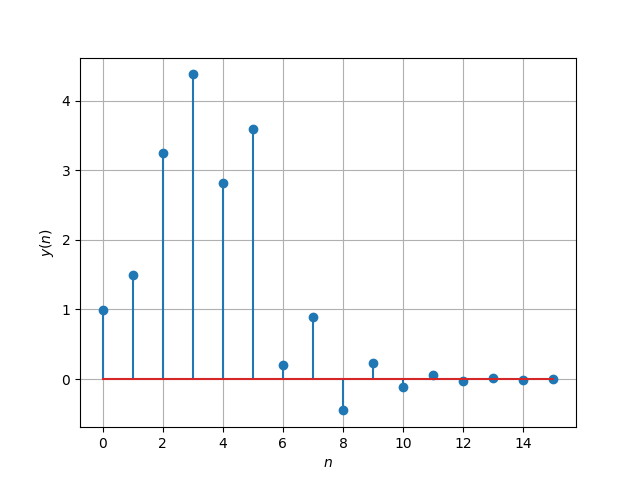
\includegraphics[width=\columnwidth]{figs/6_5.png}
	\caption{$y(n)$ using the DFT matrix}
	\label{fig:yn-mtx}
\end{figure}

\section{Exercises}
\noindent Answer the following questions by looking at the python code in Problem \ref{prob:output}.
\begin{enumerate}[label=\thesection.\arabic*]
\item
The command
\begin{lstlisting}
output_signal = signal.lfilter(b, a, input_signal)
\end{lstlisting}
in Problem \ref{prob:output} is executed through the following difference equation
\begin{equation}
\label{eq:iir_filter_gen}
 \sum _{m=0}^{M}a\brak{m}y\brak{n-m}=\sum _{k=0}^{N}b\brak{k}x\brak{n-k}
\end{equation}
where the input signal is $x(n)$ and the output signal is $y(n)$ with initial values all 0. Replace
\textbf{signal.filtfilt} with your own routine and verify.

\solution
The implementation is at
\begin{lstlisting}
$ wget https://raw.githubusercontent.com/goats-9/ee3900-assignments/main/Assignment_01/codes/7_1.py
\end{lstlisting}
and can be run using
\begin{lstlisting}
$ python3 7_1.py
\end{lstlisting}
\item Repeat all the exercises in the previous sections for the above $a$ and $b$.

\solution
%\begin{align}
%	\mtx{a} =
%	\begin{pmatrix}
%		4.44 \\ 8.78 \\ -9.93 \\ 6.90 \\ -2.93 \\ 0.70 \\ -0.07
%	\end{pmatrix}
%	\mtx{b} = 
%	\begin{pmatrix}
%		5.02 \times 10^{-5} \\ 3.52 \times 10^{-4} \\ 1.05 \times 10^{-3} \\ 1.76 \times 10^{-3} \\ 1.76 \times 10^{-3} \\ 1.05 \times 10^{-3} \\ 3.52 \times 10^{-4} \\ 5.02 \times 10^{-5} 
%	\end{pmatrix}
%\end{align}
For the given values, the difference equation is
\begin{align}
	&y(n) - \brak{4.44}y(n - 1) + \brak{8.78}y(n - 2) \nonumber \\
	&- \brak{9.93}y(n - 3) + \brak{6.90}y(n - 4) \nonumber \\
	&- \brak{2.93}y(n - 5) \nonumber + \brak{0.70}y(n - 6) \nonumber \\
	&- \brak{0.07}y(n - 7) = \brak{5.02 \times 10^{-5}}x(n) \nonumber \\
	&+ \brak{3.52 \times 10^{-4}}x(n - 1) + \brak{1.05 \times 10^{-3}}x(n - 2) \nonumber \\
	&+ \brak{1.76 \times 10^{-3}}x(n - 3) + \brak{1.76 \times 10^{-3}}x(n - 4) \nonumber \\
	&+ \brak{1.05 \times 10^{-3}}x(n - 5) + \brak{3.52 \times 10^{-4}}x(n - 6) \nonumber \\
	&+ \brak{5.02 \times 10^{-5}}x(n - 7)
\end{align}
From \eqref{eq:iir_filter_gen}, we see that the transfer function can be written as follows
\begin{align}
	H(z) &= \frac{\sum_{k = 0}^{N}b(k)z^{-k}}{\sum_{k = 0}^{M}a(k)z^{-k}} \\
		 &= \sum_{i}\frac{r(i)}{1 - p(i)z^{-1}} + \sum_{j}k(j)z^{-j}
	\label{eq:trans-func}
\end{align}
where $r(i)$, $p(i)$, are called residues and poles respectively of the partial 
fraction expansion of $H(z)$. $k(i)$ are the coefficients of the direct polynomial 
terms that might be left over. We can now take the inverse $z$-transform of
\eqref{eq:trans-func} and get using \eqref{eq:anun},
\begin{align}
	h(n) &= \sum_{i}r(i)[p(i)]^nu(n) + \sum_{j}k(j)\delta(n - j)
	\label{eq:h-n-expr}
\end{align}
Substituting the values,
\begin{align}
	&h(n) = [\brak{2.76}\brak{0.55}^n \nonumber \\ 
	&+ \brak{-1.05-1.84\j}\brak{0.57+0.16\j}^n \nonumber \\
	&+ \brak{-1.05+1.84\j}\brak{0.57-0.16\j}^n \nonumber \\
	&+ \brak{-0.53+0.08\j}\brak{0.63+0.32\j}^n \nonumber \\
	&+ \brak{-0.53-0.08\j}\brak{0.63-0.32\j}^n \nonumber \\
	&+ \brak{0.20+0.004\j}\brak{0.75+0.47\j}^n \nonumber \\
	&+ \brak{0.20-0.004\j}\brak{0.75-0.47\j}^n]u(n) \nonumber \\
	&+ \brak{-6.81 \times 10^{-4}}\delta(n)
\end{align}
The values $r(i)$, $p(i)$, $k(i)$ and thus the impulse response function are computed and plotted at
\begin{lstlisting}
$ wget https://raw.githubusercontent.com/goats-9/ee3900-assignments/main/Assignment_01/codes/7_2_1.py
\end{lstlisting}
The filter frequency response is plotted at
\begin{lstlisting}
$ wget https://raw.githubusercontent.com/goats-9/ee3900-assignments/main/Assignment_01/codes/7_2_2.py
\end{lstlisting}
Observe that for a series $t_n = r^n$, $\frac{t_{n + 1}}{t_n} = r$.
By the ratio test, $t_n$ converges if $|r| < 1$. We observe that for all $i$, 
$|p(i)| < 1$ and so, as $h(n)$ is the sum of many convergent series,
we see that $h(n)$ converges and is bounded. From \eqref{eq:z_trans},
\begin{align}
	\sum_{n = 0}^{\infty}h(n) = H(1) = \frac{\sum_{k = 0}^{N}b(k)}{\sum_{k = 0}^{M}a(k)} = 1 < \infty
\end{align}
Therefore, the system is stable. From
Fig. \eqref{fig:butter-imp}, $h(n)$ is negligible after $n \geq 64$, and we
can apply a 64-bit FFT to get y(n). The following code uses the DFT matrix
to generate $y(n)$ in Fig. \eqref{fig:butter-out}.
\begin{lstlisting}
$ wget https://raw.githubusercontent.com/goats-9/ee3900-assignments/main/Assignment_01/codes/7_2_3.py
\end{lstlisting}
The codes can be run all at once by typing
\begin{lstlisting}
$ python3 7_2_*.py
\end{lstlisting}

\begin{figure}[!htb]
	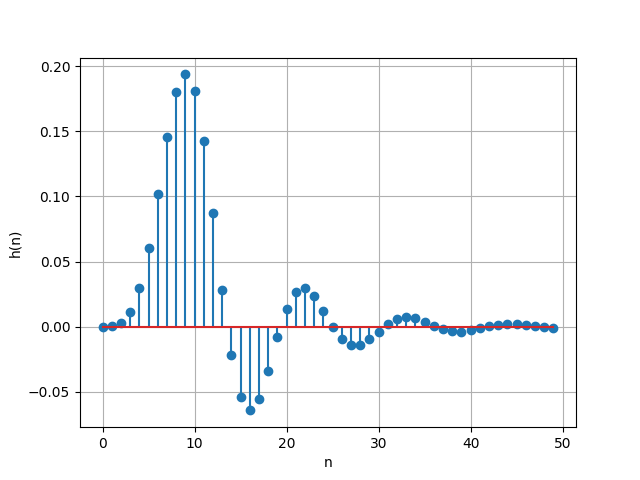
\includegraphics[width=\columnwidth]{figs/7_2_1.png}
	\caption{Plot of $h(n)$}
	\label{fig:butter-imp}
\end{figure}

\begin{figure}[!htb]
	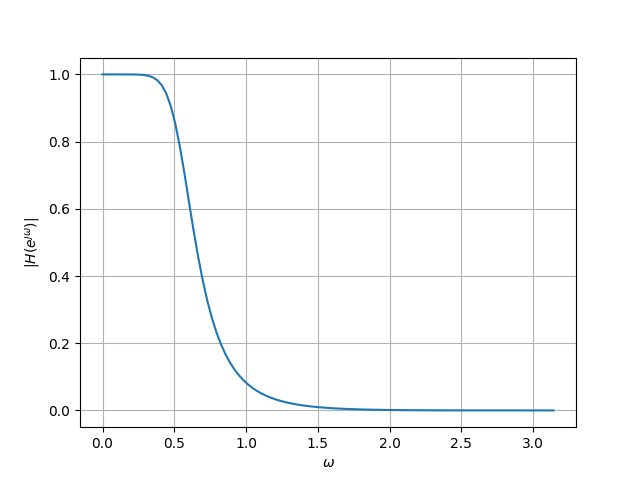
\includegraphics[width=\columnwidth]{figs/7_2_2.png}
	\caption{Filter frequency response}
	\label{fig:butter-resp}
\end{figure}

\begin{figure}[!htb]
	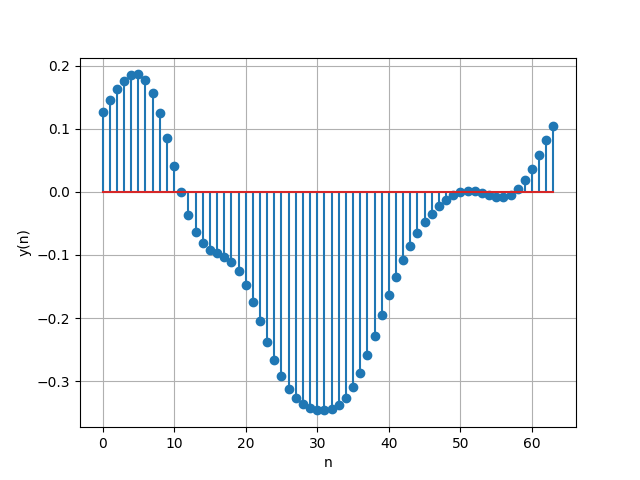
\includegraphics[width=\columnwidth]{figs/7_2_3.png}
	\caption{Plot of $y(n)$}
	\label{fig:butter-out}
\end{figure}

\item What is the sampling frequency of the input signal?

\solution
Sampling frequency $f_s = 44.1$ kHZ.
\item
What is type, order and  cutoff frequency of the above Butterworth filter?

\solution
The given Butterworth filter is low pass with order 4 and cutoff frequency 4 kHz.
\item
Modifying the code with different input parameters and to get the best possible output.

\solution
A better filtering was found on setting the order of the filter to be 7.
\end{enumerate}

\end{document}
